%!TEX TS-program = xelatex
\documentclass[xetex]{beamer}

\usefonttheme{professionalfonts}

\usepackage[UTF8]{ctex}
\usepackage{hyperref}
\usepackage{unicode-math}
\usepackage{amsmath, amssymb}
\usepackage{graphicx, wrapfig}
\usepackage{subcaption}
\usepackage{nopageno}
\usepackage{animate}

\DeclareSymbolFont{yhlargesymbols}{OMX}{yhex}{m}{n}
\DeclareMathAccent{\wideparen}{\mathord}{yhlargesymbols}{"F3}

\usetheme[block=fill]{metropolis}

\setmathfont{XITS Math}

\renewcommand{\qedsymbol}{\ensuremath{\blacksquare}}
\renewcommand{\footnotesize}{\tiny}

\title{曲线和曲面积分 II}
\subtitle{二型曲线和曲面积分}
\author{数学分析MOOC小组}
\date{}

\begin{document}
    \frame{\maketitle}

    \begin{frame}
        \frametitle{第一型 vs. 第二型}
    
        一般而言,第一型的积分是在\alert{标量场}(\alert{梯度场})中进行的,积分的对象是\alert{梯度的值}。\pause

        对应的,第二型的积分是在\alert{向量场}(\alert{矢量场})中进行的。\pause

        所以,在进行第二型积分的时候,向量的方向必须考虑在内,进行积分的对象是\alert{向量之间的内积}。
    
    \end{frame}

    \begin{frame}
        \frametitle{仍有疑问?}
    
        参见书中的规范化定义是个好主意。
    
    \end{frame}

    \section{第二型曲线积分}

    \begin{frame}
        \frametitle{定义}
    
        \begin{block}{第二型曲线积分 · 其一}
            设函数$f(x,y,z)$定义在空间光滑曲线弧$L$上,$L$的两端点为$A$,$B$。从$A$向$B$给$\wideparen{AB}$一个分法:$A=M_0,M_1,\cdots,M_n=B$,其中$M_i=(z_i,y_i,z_i)$,记$\wideparen{M_{i-1}M_i}$的弧长为$\Delta s_i$,$\Delta x_i=x_i-x_{i-1}$,任取$(\xi_i,\eta_i,\zeta_i)\in\wideparen{M_{i-1}M_i}$,作和式$$\sigma=\sum_{i=1}^nf(\xi_i,\eta_i,\zeta_i)\Delta x_i$$
            若当$\displaystyle\lambda=\max_{1\leq i\leq n}\left\{\Delta s_i\right\}\to 0$时,$\sigma$的极限存在,则称该极限为\alert{函数$f$沿有向曲线$L$对$x$的第二型曲线积分},记为$$\int_Lf(x,y,z)\,\mathrm{d}x\text{ 或 }\int_{\wideparen{AB}}f(x,y,z)\,\mathrm{d}x$$
        \end{block}
    
    \end{frame}

    \begin{frame}
        \frametitle{定义}
    
        \begin{block}{第二型曲线积分 · 其二}
            使用类似的方法,还可以定义\alert{函数$f$沿有向曲线$L$对$y$或对$z$的第二型曲线积分}为$$\int_Lf(x,y,z)\,\mathrm{d}y$$或$$\int_Lf(x,y,z)\,\mathrm{d}z$$
        \end{block}
    
    \end{frame}

    \begin{frame}
        \frametitle{定义}
    
        \begin{block}{第二型曲线积分 · 其三}
            如果有\alert{向量函数}$\mathbf{F}(x,y,z)=\left(P(x,y,z),Q(x,y,z),R(x,y,z)\right)$,则记
            $$\begin{aligned}
                & \int_LP(x,y,z)\,\mathrm{d}x+\int_LQ(x,y,z)\,\mathrm{d}y+\int_LR(x,y,z)\,\mathrm{d}z \\
                = & \lim_{\lambda\to 0}\sum_{i=1}^n\left[P(\xi_i,\eta_i,\zeta_i)\Delta x_i+Q(\xi_i,\eta_i,\zeta_i)\Delta y_i+R(\xi_i,\eta_i,\zeta_i)\Delta z_i\right]
            \end{aligned}$$
            其中$\Delta x_i$,$\Delta y_i$,$\Delta z_i$分别是向量$\overrightarrow{M_{i-1}M_i}$在$x$,$y$,$z$轴上的有向投影。
        \end{block}
    
    \end{frame}

    \begin{frame}
        \frametitle{定义}
    
        \begin{block}{第二型曲线积分 · 其四}
            若记$$\mathrm{d}\mathbf{s}=\left\{\mathrm{d}x,\mathrm{d}y,\mathrm{d}z\right\}$$
            则$$\begin{aligned}
                & \int_LP(x,y,z)\,\mathrm{d}x+\int_LQ(x,y,z)\,\mathrm{d}y+\int_LR(x,y,z)\,\mathrm{d}z \\
                = & \int_L\mathbf{F}(x,y,z)\cdot\mathrm{d}\mathbf{s}
            \end{aligned}$$
            因此上述积分也称为向量函数$\mathbf{F}(x,y,z)$\alert{沿有向曲线$L$的积分}。$\mathrm{d}\mathbf{s}$的方向就是曲线$L$的\alert{切线方向},其指向\alert{与$L$的方向一致}。
        \end{block}
    
    \end{frame}

    \begin{frame}
        \frametitle{定义}
    
        \begin{block}{第二型曲线积分 · 其五}
            若曲线$L$为\alert{闭曲线},上述积分还记作
            $$\oint_LP\,\mathrm{d}x+Q\,\mathrm{d}y+R\,\mathrm{d}z$$
            该积分的值只与$L$的方向有关,与积分的起点之位置无关。
        \end{block}
    
    \end{frame}

    \begin{frame}
        \frametitle{图解}
        \begin{figure}[ht]
            \centering
            \animategraphics[loop, autoplay, width=.5\linewidth, timeline=img/Line_integral_of_vector_field/Line_integral_of_vector_field.txt]{10}{img/Line_integral_of_vector_field/Line_integral_of_vector_field-}{0}{130}
            \caption{动图理解第二型曲线积分\footnote[1]{\href{https://commons.wikimedia.org/wiki/File:Line_integral_of_vector_field.gif}{本图由作者Lucas Vieira释出于公有领域}}}
        \end{figure}
    
    \end{frame}

    \begin{frame}
        \frametitle{计算}
    
        设$f(x,y,z)$是定义在光滑曲线段
        $$\wideparen{AB}:x=x(t),y=y(t),z=z(t),\quad \alpha\leq t\leq\beta$$
        上的连续函数,$t=\alpha$时对应于$A$点,$t=\beta$时对应于$B$点,且$\wideparen{AB}$自身不相交,则有
        $$\int_{\wideparen{AB}}f(x,y,z)\,\mathrm{d}x=\int_\alpha^\beta f\left(x(t),y(t),z(t)\right)x^\prime(t)\,\mathrm{d}t$$
        类似的还可以得到$\displaystyle\int_{\wideparen{AB}}f(x,y,z)\,\mathrm{d}y$和$\displaystyle\int_{\wideparen{AB}}f(x,y,z)\,\mathrm{d}z$的表达式,将三者加起来就可以了。\pause 这将第二型曲线积分转化为了\alert{普通积分}之和。
    
    \end{frame}

    \begin{frame}
        \frametitle{将第二型转换为第一型}
    
        记上述曲线段的切向量$\boldsymbol{\tau}=\left(x^\prime(t),y^\prime(t),z^\prime(t)\right)$。当然,这个切向量是一个关于$t$的函数,代表了曲线上不同点处的切向量方向。
        则有
        $$\begin{aligned}
            & \int_{\wideparen{AB}}P\,\mathrm{d}x+Q\,\mathrm{d}y+R\,\mathrm{d}z \\
            = & \int_{\wideparen{AB}}\left[P\cos(\boldsymbol{\tau},x)+Q\cos(\boldsymbol{\tau},y)+R\cos(\boldsymbol{\tau},z)\right]\,\mathrm{d}t
        \end{aligned}$$
        其中$\cos(\boldsymbol{\tau},x)$代表向量$\boldsymbol{\tau}$与$x$正方向之夹角之余弦值,$\cos(\boldsymbol{\tau},y)$和$\cos(\boldsymbol{\tau},z)$含义类似。\pause

        这两种计算方法都是很基础很常见的计算方法,都应当掌握。
    
    \end{frame}

    \section{第二型曲面积分}

    \begin{frame}
        \frametitle{定义}
    
        \begin{block}{第二型曲面积分 · 其一}
            设函数$f(x,y,z)$定义在光滑的双侧曲面$S$上。给定$S$的一侧,这等于指定了$S$上每一点的单位法向量$\mathbf{n}(x,y,z)=(\cos\alpha,\cos\beta,\cos\gamma)$。任给$S$一个分法$\Delta S_i$,$i=1,2,\cdots,n$,其中$\Delta S_i$既表示小块曲面,也表示曲面的面积。在$\Delta S_i$中任取$(\xi_i,\eta_i,\zeta_i)$,记$\Delta D_i$为$\Delta S_i$在$Oxy$平面的有向投影,即$\Delta D_i=\Delta S_i\cos\gamma_i$,其中$\cos\gamma_i$是$\cos\gamma$在$(\xi_i,\eta_i,\zeta_i)$点的值。作和
            $$\sum_{i=1}^nf(\xi_i,\eta_i,\zeta_i)\Delta D_i$$

        \end{block}
    
    \end{frame}

    \begin{frame}
        \frametitle{定义}
    
        \begin{block}{第二型曲面积分 · 其二}
            若当$\displaystyle\lambda=\max_{1\leq i\leq n}\left(\mathrm{d}(\Delta S_i)\right)\to 0$时,上述和式的极限存在,则称这极限为\alert{$f$在曲面指定侧对$x$,$y$的第二型曲面积分},记为$$\iint_Sf(x,y,z)\,\mathrm{d}x\mathrm{d}y$$
            类似的,可以定义以下两个曲面积分
            $$\iint_Sf(x,y,z)\,\mathrm{d}y\mathrm{d}z\text{ 和 }\iint_Sf(x,y,z)\,\mathrm{d}z\mathrm{d}x$$
        \end{block}
    
    \end{frame}

    \begin{frame}
        \frametitle{定义}
    
        \begin{block}{第二型曲面积分 · 其三}
            假如我们的向量函数还是$\mathbf{F}(x,y,z)=\left(P(x,y,z),Q(x,y,z),R(x,y,z)\right)$,那么所谓的\alert{流量}就是这三个曲面积分之和
            $$\iint_SP\,\mathrm{d}y\mathrm{d}z+Q\,\mathrm{d}z\mathrm{d}x+R\,\mathrm{d}x\mathrm{d}y$$
        \end{block}
    
    \end{frame}

    \begin{frame}
        \frametitle{定义}
    
        \begin{block}{第二型曲面积分 · 其四}
            与第二型曲线积分类似,若记
            $$\begin{aligned}
                \mathrm{d}\mathbf{S} &= \mathbf{n}\cdot\mathrm{d}S=\left\{\cos\alpha,\cos\beta,\cos\gamma\right\}\mathrm{d}S \\
                &= \left\{\mathrm{d}y\mathrm{d}z,\mathrm{d}z\mathrm{d}x,\mathrm{d}x\mathrm{d}y\right\}
            \end{aligned}$$
            则
            $$\begin{aligned}
                & \iint_SP\,\mathrm{d}y\mathrm{d}z+Q\,\mathrm{d}z\mathrm{d}x+R\,\mathrm{d}x\mathrm{d}y \\
                = & \iint_S(P\cos\alpha+Q\cos\beta+R\cos\gamma)\,\mathrm{d}S \\
                = & \iint_S\mathbf{F}\cdot\mathrm{d}\mathbf{S}
            \end{aligned}$$
            这里$\mathrm{d}\mathbf{S}$的方向为法线方向,与积分曲面$S$的侧相同。
        \end{block}
    
    \end{frame}

    \begin{frame}
        \frametitle{图解}
    
        \begin{figure}[ht]
            \centering
            \begin{subfigure}[b]{.4\textwidth}
                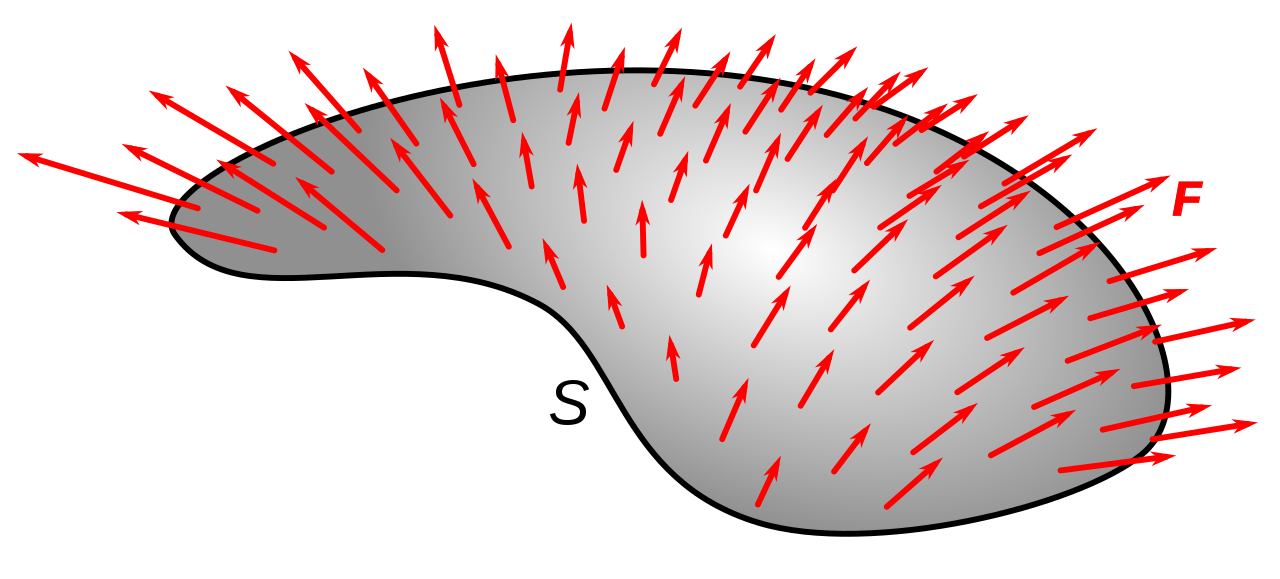
\includegraphics[width=\textwidth]{img/1280px-Surface_integral_-_vector_field_thru_a_surface.svg}
                \caption{曲面上的向量场}
                \label{fig:intplate-1a}
            \end{subfigure}
            ~
            \begin{subfigure}[b]{.4\textwidth}
                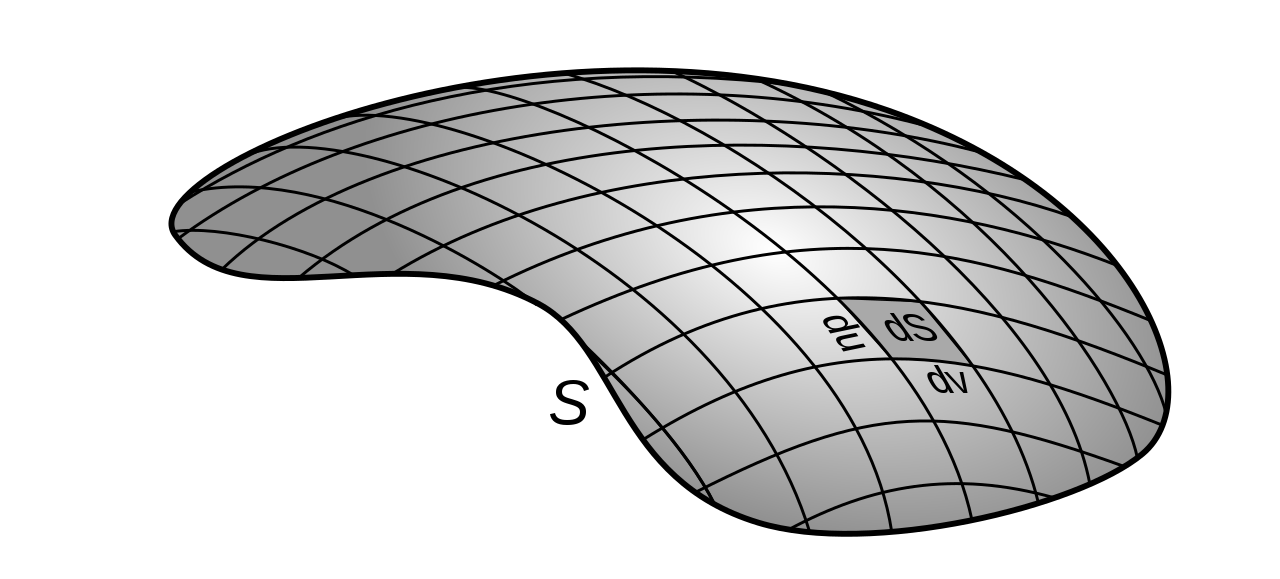
\includegraphics[width=\textwidth]{img/1280px-Surface_integral_-_parametrized_surface.svg.png}
                \caption{曲面细分为多个小块}
                \label{fig:intplate-1b}
            \end{subfigure}
            \caption{第二型曲面积分 · 其一\footnote[1]{\href{https://commons.wikimedia.org/wiki/File:Surface_integral_-_vector_field_thru_a_surface.svg}{图\ref{fig:intplate-1a}由作者Chetvorno以CC0 1.0协议公开}}\footnote[2]{\href{https://commons.wikimedia.org/wiki/File:Surface_integral_-_parametrized_surface.svg}{图\ref{fig:intplate-1b}由作者Chetvorno以CC0 1.0协议公开}}}
            \label{fig:intplate-1}
        \end{figure}
    
    \end{frame}

    \begin{frame}
        \frametitle{图解}
    
        \begin{figure}[ht]
            \centering
            \begin{subfigure}[b]{.4\textwidth}
                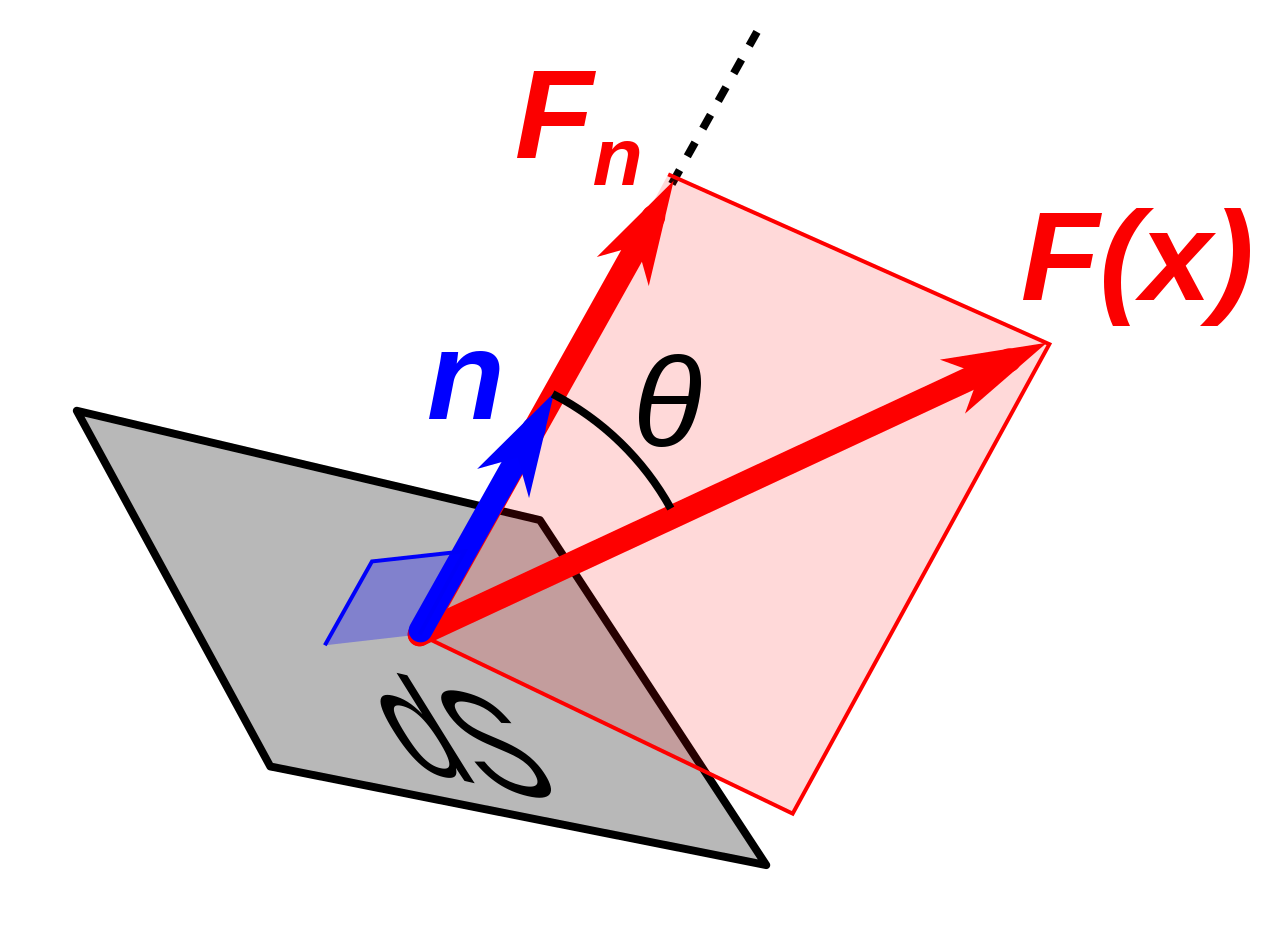
\includegraphics[width=\textwidth]{img/1280px-Surface_integral_-_normal_component_of_field.svg.png}
                \caption{每个小块的流量}
                \label{fig:intplate-2a}
            \end{subfigure}
            ~
            \begin{subfigure}[b]{.4\textwidth}
                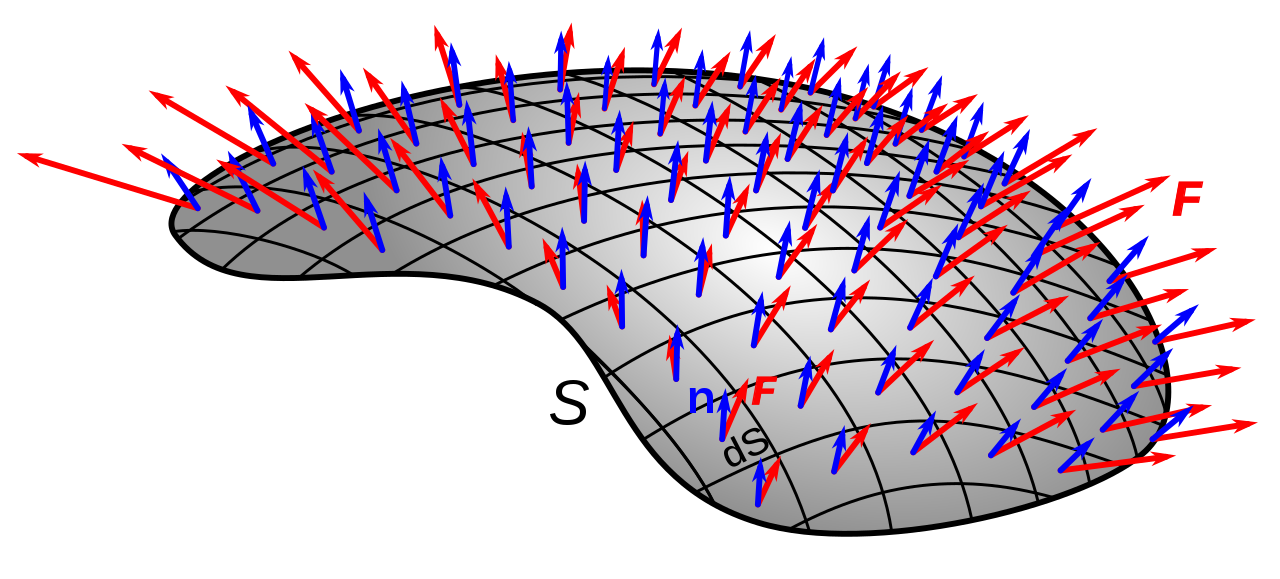
\includegraphics[width=\textwidth]{img/1280px-Surface_integral_-_definition.svg.png}
                \caption{整个曲面的流量}
                \label{fig:intplate-2b}
            \end{subfigure}
            \caption{第二型曲面积分 · 其二\footnote[1]{\href{https://commons.wikimedia.org/wiki/File:Surface_integral_-_normal_component_of_field.svg}{图\ref{fig:intplate-2a}由作者Chetvorno以CC0 1.0协议公开}}\footnote[2]{\href{https://commons.wikimedia.org/wiki/File:Surface_integral_-_definition.svg}{图\ref{fig:intplate-2b}由作者Chetvorno以CC0 1.0协议公开}}}
            \label{fig:intplate-1}
        \end{figure}
    
    \end{frame}

    \begin{frame}
        \frametitle{计算}
    
        设$R(x,y,z)$在光滑曲面$$S:z=z(x,y),\quad (x,y)\in D$$
        上连续,则
        $$\iint_SR(x,y,z)\,\mathrm{d}x\mathrm{d}y = \pm \iint_DR(x,y,z(x,y))\,\mathrm{d}x\mathrm{d}y$$
        其中$S$为上侧时取正号,$S$为下侧时取负号。
    
    \end{frame}

    \begin{frame}
        \frametitle{计算}
    
        类似的还能得到
        $$\iint_SP(x,y,z)\,\mathrm{d}y\mathrm{d}z = \pm \iint_EP(x(y,z),y,z)\,\mathrm{d}y\mathrm{d}z$$
        和
        $$\iint_SQ(x,y,z)\,\mathrm{d}z\mathrm{d}x = \pm \iint_GQ(x,y(x,z),z)\,\mathrm{d}z\mathrm{d}x$$
        其中$E$和$G$分别为$S$在$Oyz$和$Ozx$平面的投影。\pause

        流量是上述三者之和,这将第二型曲面积分转化为了\alert{重积分}之和。
    
    \end{frame}

    \begin{frame}
        \frametitle{其他计算法}
    
        你也可以利用
        $$\begin{aligned}
            & \iint_SP\,\mathrm{d}y\mathrm{d}z+Q\,\mathrm{d}z\mathrm{d}x+R\,\mathrm{d}x\mathrm{d}y \\
            = & \iint_S(P\cos\alpha+Q\cos\beta+R\cos\gamma)\,\mathrm{d}S
        \end{aligned}$$
        来将第二型曲面积分转化为\alert{第一型曲面积分}来计算。
    
    \end{frame}

    \section{FAQ}

    \begin{frame}
        \frametitle{我分不清第二型曲面积分与重积分了!}
    
        这是第二型曲面积分
        $$\iint_SP(x,y,z)\,\mathrm{d}y\mathrm{d}z$$\pause
        这是对应的重积分
        $$\iint_EP(x(y,z),y,z)\,\mathrm{d}y\mathrm{d}z$$\pause

        重积分当中,被积函数的变量\alert{全部都出现}在了微元部分当中,但是第二型积分的被积函数多了一个变量$x$。
    
    \end{frame}

    \begin{frame}
        \frametitle{我能分清第一型曲线积分与普通积分了!}
    
        对比第一型曲线积分和普通积分
        $$\int_{\wideparen{AB}}f(x,y,z)\,\mathrm{d}x$$\pause
        $$\int_\alpha^\beta f\left(x(t),y(t),z(t)\right)x^\prime(t)\,\mathrm{d}t$$\pause

        普通积分当中,被积函数的变量只有一个$t$,但是第二型积分的被积函数的变量足足有$x$、$y$、$z$三个之多。
    
    \end{frame}

    \section{例题}

    \begin{frame}
        \frametitle{例题}
        \centering
        没有例题
    
    \end{frame}

    \begin{frame}
        \frametitle{例题}
        \centering
        真正的挑战需要等到下一章才会开启
    
    \end{frame}

    \begin{frame}
        \frametitle{例题}
        \centering
        学着书上的例题死算就会了
    
    \end{frame}

    \begin{frame}[standout]
    
        感谢

        \small{曲线和曲面积分 II · 终}
    
    \end{frame}
\end{document}
